\documentclass[letter, 10pt]{article}
\usepackage[utf8]{inputenc}
\usepackage[spanish]{babel}
\usepackage{amsfonts}
\usepackage{amsmath}
\usepackage[dvips]{graphicx}
\usepackage{graphicx}
\usepackage{subfigure} % subfiguras
\DeclareGraphicsExtensions{.bmp,.png,.pdf,.jpg}
\usepackage{xcolor,listings}%color support for listings
\usepackage{epstopdf}
\usepackage{algpseudocode}
\usepackage{algorithm}
\usepackage{url}
\usepackage{caption}
\usepackage[top=3cm,bottom=3cm,left=3.5cm,right=3.5cm,footskip=1.5cm,headheight=1.5cm,headsep=.5cm,textheight=3cm]{geometry}



\begin{document}



\title{Análisis Inteligente de Datos \\ \begin{Large}Tarea 1\end{Large}}
\author{Paulina Aguila - Anibal Pérez}
\date{28 de abril de 2016}

\maketitle


\begin{figure}[ht]
\begin{center}

\includegraphics[width=0.2\textwidth]{Images/Isotipo-Negro.png}\\
\end{center}
\end{figure}
\vspace{2cm}
\section{Introducci\'on}
Este documento busca poner en práctica los métodos de análisis de datos utilizados y estudiados en clases. Para ello, se dispondrá de 2 conjuntos de datos diferentes. El primero se centrará en la manipulación de Dataframes, mientras que el segundo en el método conocido como PCA. En ambos se tratará la visualización de datos y resultados.\\

Para los dos problemas propuestos, se realizará una implementación computacional utilizando un entorno Windows 7 y Python como el lenguaje de programación escogido, en donde se utilizarán librerías como numpy, pandas, sklearn, entre otras.\\

Al final de la experiencia, se espera obtener resultados concretos que logren responder las preguntas propuestas basándose en el análisis de datos a través de su implementación computacional.

\section{Manipulación Básica de Dataframes y Visualización I}

Para esta primera sección, se estudiará el caso de TITANIC, el conocido transatlántico británico que se hundió en su viaje inaugural el año 1912, en el cual murieron cerca de 1502 personas. Al finalizar el análisis de los datos que se tienen sobre el TITANIC, se espera responder las siguientes preguntas: ¿Qué pasajeros tenían mayor probabilidad de sobrevivir? ¿Es posible predecir quién se salvaría y quién no?

\subsection{Descripción de los datos}

En primer lugar, se determinó que se tienen 11 variables y 891 datos. Las variables son las siguientes \cite{W1}:

\begin{itemize}
\item \textbf{Survived:} variable categórica nominal que representa si el individuo sobrevivió o no a la tragedia. Toma los siguientes valores: 0: No sobrevivió - 1: Sí sobrevivió. No hay datos faltantes.
\item \textbf{Pclass:} variable categórica ordinal que representa la clase del pasajero en la embarcación. Toma los siguientes valores: 1: Primera clase - 2: Segunda clase - 3: Tercera Clase. Es un indicador del estatus socioeconómico del individuo, en donde 1era clase es más alta que la 2da, siendo la 3era la más baja. No hay datos faltantes.
\item\textbf{Name:} Variable categórica nominal que contiene el nombre del individuo. Todos los valores son distintos entre sí al tratarse de un nombre. No hay datos faltantes.
\item \textbf{Sex:} Variable categórica nominal que representa el sexo del individuo. Toma los siguientes valores: male: hombre - female: mujer. No hay datos faltantes.
\item \textbf{Age:} Variable cuantitativa de tipo continua que representa la edad en años de la persona. Toma valores desde 0.42 hasta 80 años. Valores fraccionados de la forma 0.x corresponden a edades menores a 1 año, y de la forma xx.5 son valores estimados. Sí hay datos faltantes.
\item \textbf{Sibsp:} Variable cuantitativa discreta que contiene el número de hermanos/as y esposos/as legales que tiene el individuo abordo del TITANIC. Toma valores entre 0 y 8. No hay datos faltantes.
\item \textbf{Parch:} Variable cuantitativa discreta que contiene el número de padres e hijos que tiene el individuo abordo del TITANIC. Toma valores entre 0 y 6. No hay datos faltantes.
\item \textbf{Ticket:} Variable -- que corresponde al número de ticket del pasajero. -- No hay datos faltantes.
\item \textbf{Fare:} Variable cuantitativa de tipo continua que representa la tarifa que pagó el pasajero por su ticket. Toma valores desde 0 a 5.123.292. No se especifica la moneda, sin embargo, se deduce que serian euros al tratarse de una embarcación británica. No hay datos faltantes.
\item \textbf{Cabin:} Variable categórica nominal que representa la cabina o habitación en la que se encontraba alojado el pasajero. Sí hay datos faltantes.
\item \textbf{Embarked:} Variable categórica nominal que representa el puerto de embarque del pasajero. Toma los siguientes valores: C: Cherbourg - Q: Queenstown - S: Southampton. Sí hay valores faltantes.
\end{itemize}

\subsection{Manipulación del dataframe}

Al tener el dataframe en Python con los datos a utilizar, se utiliza el comando data.info() para conocer más información sobre los datos, como por ejemplo, la cantidad de filas con datos no nulos y el tipo de dato que alberga la variable, ya sea si es entero, flotante u objeto. Con el comando data.describe(), se muestran datos estadísticos aplicados a variables de tipo cuantitativas, como son la media, desviación estándar, mínimo, máximo y 3 percentiles correspondientes al 25\%, 50\% y 75\%.\\

Analizando los datos de sobrevivencia en base al sexo de las personas, se obtuvo que  de un total de 577 hombres que iban en la embarcación, solo un 18,89\% sobrevivió, mientras que de un total de 314 mujeres, sobrevivieron un 74,20\%. Esta proporción se puede observar en la Figura 1.a.\\

Por otro lado, de un total de 342 personas sobrevivientes, el 68,13\% correspondían a mujeres, mientras que el 31,87\%  restante correspondían a hombres. Esta relación se ve claramente en la Figura 1.b, en donde la proporción de mujeres sobrevivientes es más del doble de la cantidad de hombres.

\begin{figure}[H]
\subfigure[Gráfico para la cantidad de sobrevivientes o fallecidos de acuerdo a su sexo]{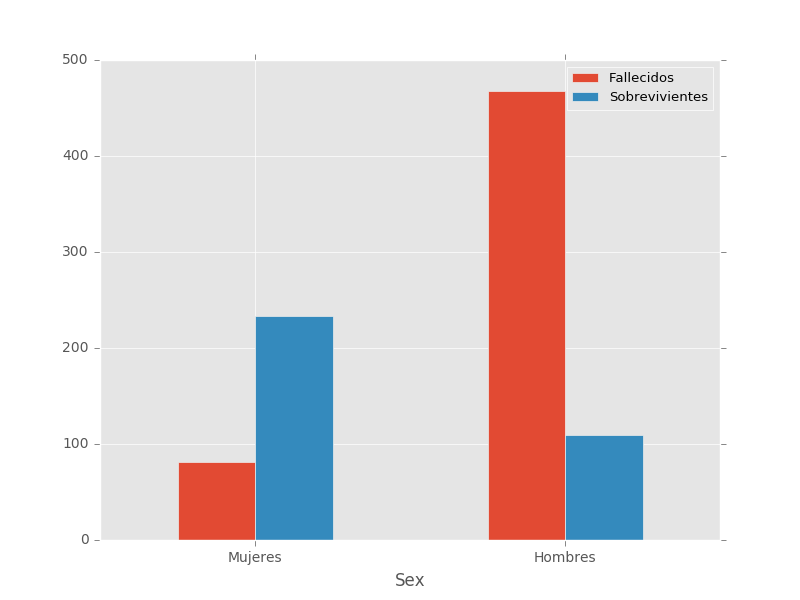
\includegraphics[width=0.5\textwidth]{Images/figure_1.png}}
\subfigure[Gráfico para la cantidad mujeres u hombres que fallecieron o sobrevivieron]{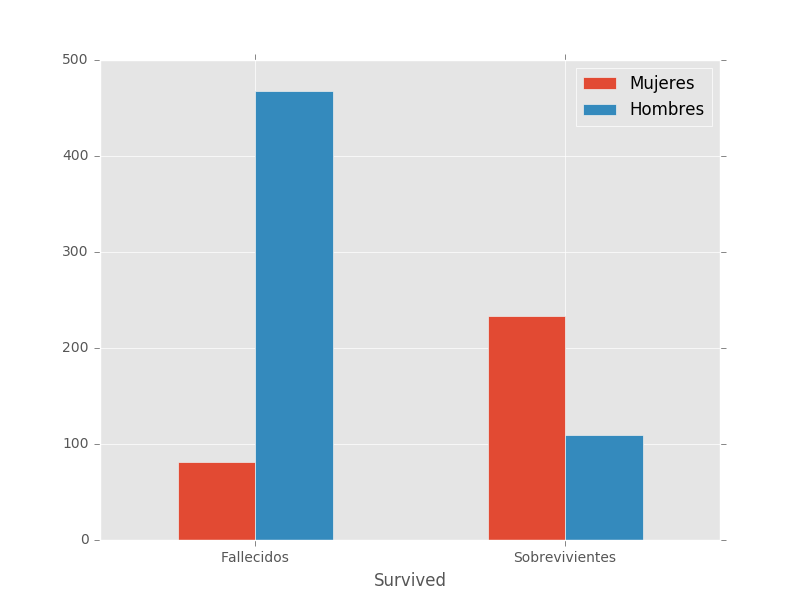
\includegraphics[width=0.5\textwidth]{Images/figure_2.png}}
\caption{Gráficos de barra que relaciona la sobrevivencia con la variable sexo.}
\end{figure}


Dado el análisis anterior, se puede decir que existe una correlación entre el género de la persona y su probabilidad de sobrevivir, ya que los datos apuntan a que las mujeres fueron las que tienen una tasa de sobrevivencia mucho mayor que la de los hombres. Esto confirma el hecho de que se haya puesto más esfuerzo en salvar a mujeres llevándoselas en botes salvavidas que a hombres.\\

Al estudiar la relación de la sobrevivencia con las edades de los individuos, se obtuvo que la edad media de sobrevivientes fue de 28 años, mientras que los fallecidos tenían en promedio 30 años. Dichos valores no muestran una clara correlación entre la edad y el hecho de sobrevivir, por lo que se requiere algún análisis más detallado. Para esto se hizo un histograma de la cantidad de sobrevivientes y fallecidos de acuerdo a las edades, el cual se muestra en la Figura 2.\\

\begin{figure}[h]
\begin{center}
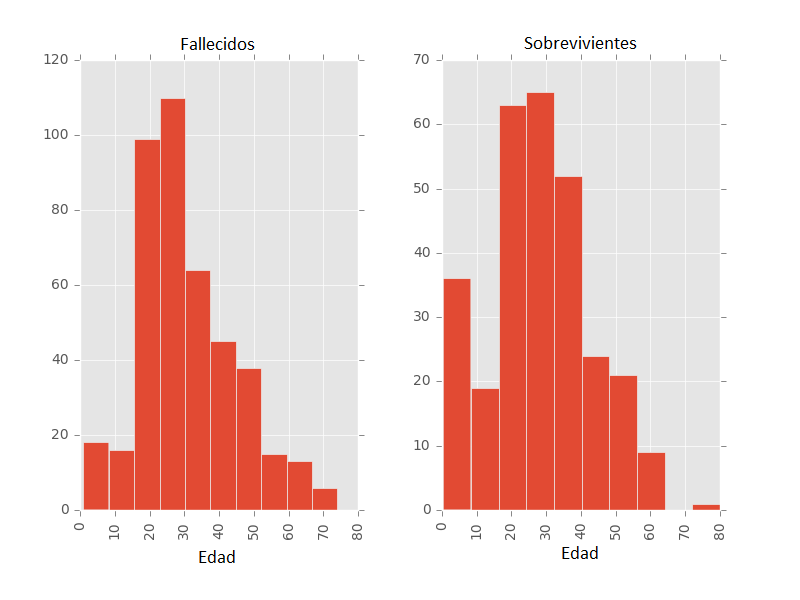
\includegraphics[width=0.7\textwidth]{Images/figure_4.png}
\caption{Histograma correspondiente a la cantidad de fallecidos y sobrevivientes de acuerdo a la variable edad.}
\end{center}
\end{figure}

De la Figura 2 se puede observar que sobrevivieron más personas menores a 40 años. Sin embargo, una tendencia muy parecida se observa en el gráfico de fallecidos, de igual forma se aprecia que sobrevivieron una mayor cantidad de niños que los que murieron. Por otro lado, se puede ver que el pasajero más adulto abordo tenía una edad de 80 años, quien sobrevivió al naufragio.\\

Para un mayor análisis se realizó un gráfico de caja (boxplot) con la misma información, el que se puede ver en la Figura 3. Dicho gráfico, confirma las conclusiones realizadas, mostrando los outliers o valores poco frecuentes que pueden haber modificado los histogramas.\\

De ambas figuras, se aprecia que existe una correlación entre la sobrevivencia y la edad poco marcada, ya que es el mismo rango de edad en que existe la mayor cantidad de personas tanto fallecidas como sobrevivientes.

\begin{figure}[H]
\begin{center}
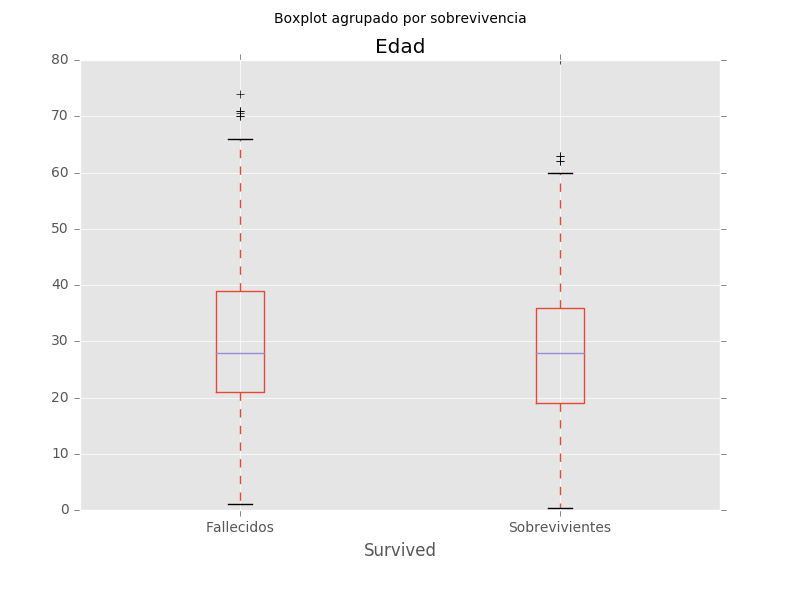
\includegraphics[width=0.7\textwidth]{Images/figure_3.png}
\caption{Gráfico de caja correspondiente a la cantidad de fallecidos y sobrevivientes de acuerdo a la variable edad.}
\end{center}
\end{figure}

Para la variable edad, se vio que existen en total 177 datos faltantes, de los cuales 125 corresponden a los fallecidos y 52 a los sobrevivientes. Este hecho influye en los resultados finales ya que corresponden aproximadamente a un 20\% de los datos totales, lo que podría entregar resultados menos fiables. Además, tomando en cuenta que la correlación de la edad con la sobrevivencia tiene una correlación bastante estrecha, puede que ese 20\% faltante cambie completamente los resultados. \\

Al reemplazar los valores nulos por el promedio de edad de las mujeres (29 años) y de los hombres (31 años)  según corresponda, se obtuvo el gráfico de caja mostrado en la Figura 4, en el cual se puede ver una diferencia con la Figura 3 en que los percentiles están más pequeños y se centran en un rango de edad cercano a los 29 y 31 años. Sin embargo, los resultados nuevos no cambiaron la tendencia ni la correlación de las variables.

\begin{figure}[H]
\begin{center}
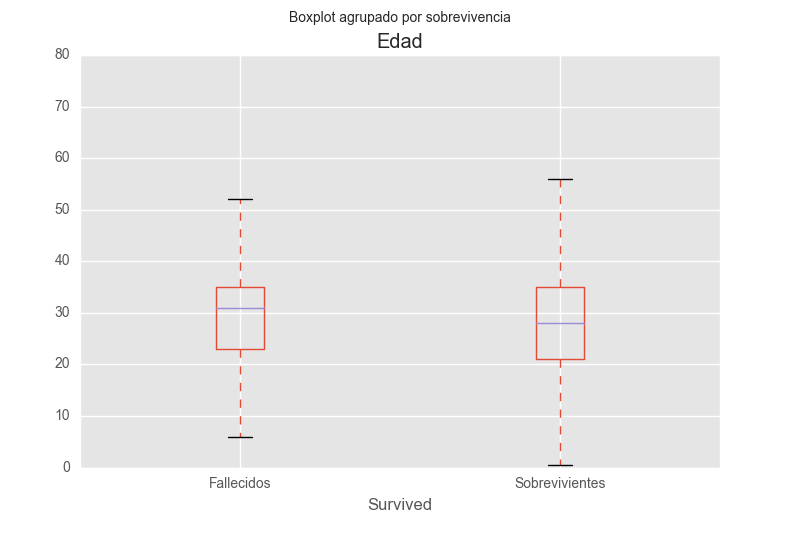
\includegraphics[width=0.7\textwidth]{Images/figure_5.png}
\caption{Gráfico de caja correspondiente a la cantidad de fallecidos y sobrevivientes de acuerdo a la variable edad, reemplazando los valores nulos por la media de la edad para hombres y mujeres.}
\end{center}
\end{figure}

En la embarcación, se podían encontrar 3 tipos de clases de pasajeros: 1era clase, 2da clase y 3era clase. Estas categorías estaban directamente relacionadas con el estatus socioeconómico del pasajero, es decir, en 1era clase se encontraban los pasajeros con mayores recursos económicos, mientras que en la 3era clase estaba la gente más pobre. \\

Al tener dicha información, se puede analizar si existe alguna relación entre la clase del pasajero y la probabilidad de sobrevivir al accidente.\\

En primer lugar, se tiene que en el naufragio sobrevivieron 342 personas de un total de 891 (total de datos), de los cuales sobrevivieron 136 personas de primera clase (39,77\%), 87 personas de segunda clase (25,44\%) y 119 personas de tercera clase (34,80\%). Por otro lado, de los pasajeros de 1era clase, sobrevivió un 62,96\%, mientras que en 2da clase sobrevivió el 47,29\%. Finalmente, en la 3era clase, sobrevivieron solo el 24,24\% de los pasajeros. Toda esta información se ve reflejada en las Figuras 5.a y 5.b.

\begin{figure}[H]
\subfigure[Proporción de cada clase que sobrevivió]{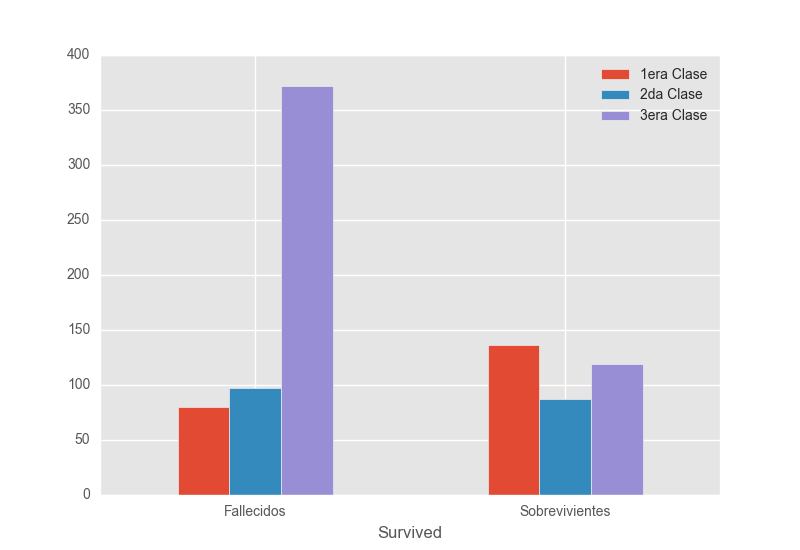
\includegraphics[width=0.5\textwidth]{Images/figure_7.png}}
\subfigure[Proporción de sobrevivientes de cada clase]{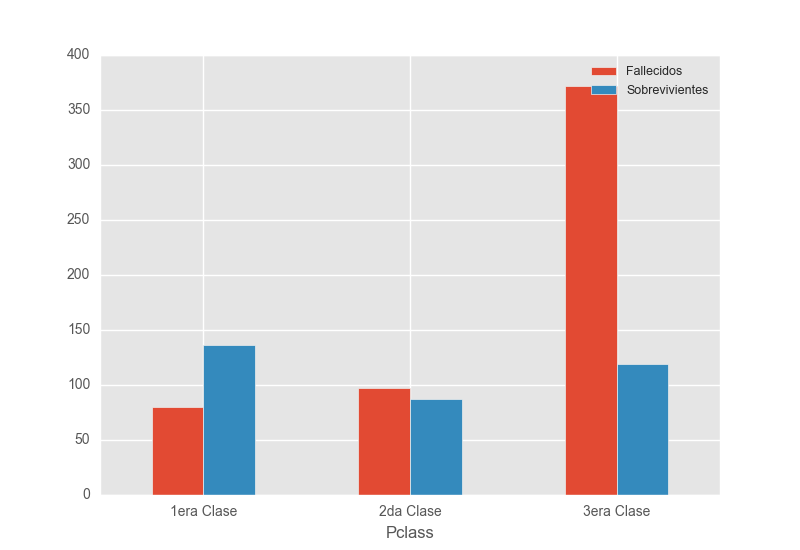
\includegraphics[width=0.5\textwidth]{Images/figure_8.png}}
\caption{Relación entre sobrevivencia y clase del pasajero en la embarcación.}
\end{figure}

Observando dichos gráficos, se puede ver que existen relaciones bastante marcadas con respecto a sobrevivir de acuerdo a la clase del pasajero. De las personas fallecidas, la mayoría de estas eran pobres, mientras que sobrevivieron más pasajeros de 1era clase. Además, de la Figura 5.b, se ve claramente que en la 3era clase hubieron más fallecidos que sobrevivientes. Por lo tanto, se establece como relación que si es un pasajero de 3era clase, éste tenía mayores probabilidades de morir que de sobrevivir, no así con los de 1era.\\

Por otro lado, se estudia la relevancia del sexo junto con la clase en la sobrevivencia del individuo. Para el caso de las mujeres que sobrevivieron, un 39,06\% era de 1era clase, un 30,04\% era de 2da y un 30,90\% era de 3era. Esta proporción se puede ver en la Figura 6.a. Para el caso de los hombres sobrevivientes, el 41,28\% viajaban en 1era clase, mientras que el 15,60\% era de 2da y 43,12\% viajaba en 3era. Esta relación se ve en la Figura 6.b.

\begin{figure}[H]
\subfigure[Proporción de sobrevivientes mujeres de cada clase]{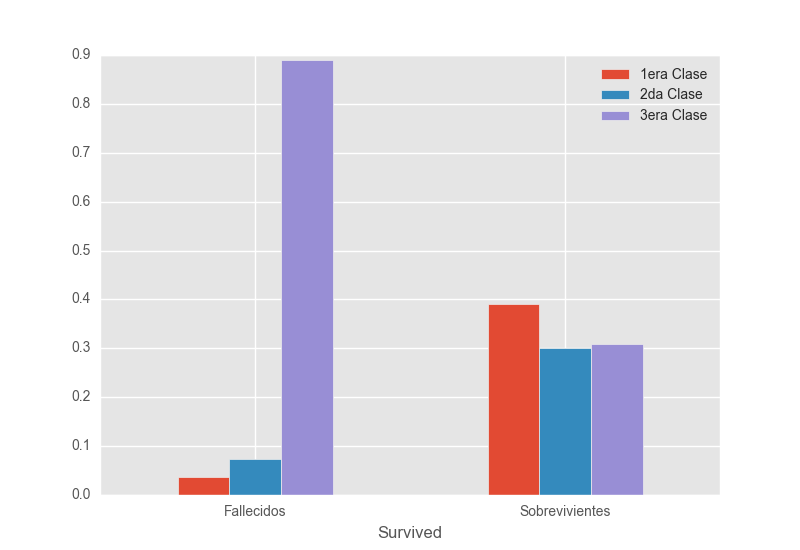
\includegraphics[width=0.5\textwidth]{Images/figure_6.png}}
\subfigure[Proporción de sobrevivientes hombres de cada clase]{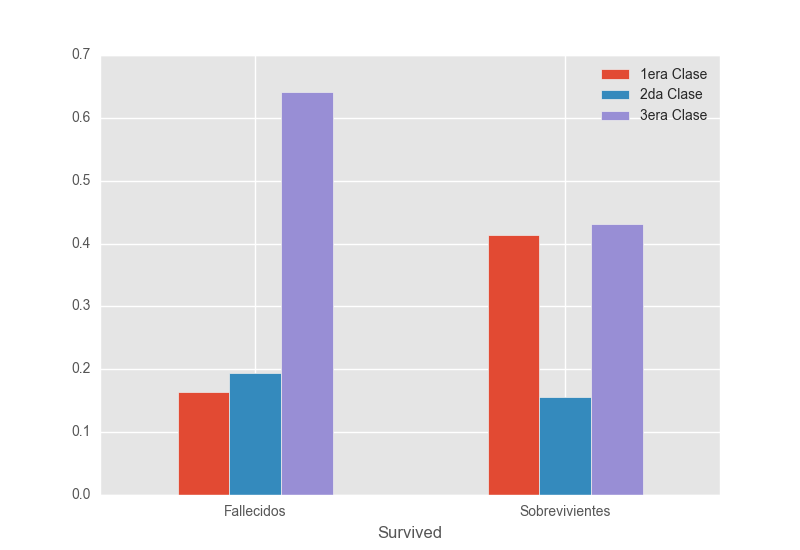
\includegraphics[width=0.5\textwidth]{Images/figure_9.png}}
\caption{Relación entre sobrevivencia y clase del pasajero en la embarcación, según su sexo.}
\end{figure}

En base a estos gráficos, se tiene que de las mujeres que fallecieron, casi el 90\% corresponde a mujeres de 3era clase,  mientras que con los hombres, pasa algo muy parecido.\\

Luego, se aplicó un método a los datos de entrenamiento (train) de tal forma que se predijera si la persona iba a sobrevivir o fallecer de acuerdo al sexo y clase del pasajero.\\

De acuerdo a los datos analizados anteriormente, se propuso la regla de que si una persona es del sexo femenino  y perteneciente a la 1era o 3era clase, ésta iba a sobrevivir, mientras que si era de sexo masculino perteneciente a la 1era clase, éste iba a sobrevivir. Esto se decidió en base a los análisis anteriores de sobrevivencia de acuerdo al sexo, en donde el 68,13\% de los sobrevivientes eran mujeres, y al relacionarlo con la clase, esta variable determinó que sobrevivían más mujeres de 1era y 3era clase. Con respecto a los hombres, se determinó que si éste pertenecía a 1era clase, tenía más probabilidades de sobrevivir.\\

Al agregar la columna de predicción al dataset de entrenamiento, se obtuvo una precisión (proporción de las veces que se predice muerte/sobrevivencia y efectivamente la persona murió/sobrevivió) de 57,77\% mientras que el recall (proporción de los muertos/sobrevivientes que su regla efectivamente predice como tales) fue de 60,82\%.\\

A continuación, se procedió a realizar un gráfico de caja para los valores que toma la variable Fare, que se refiere al precio del ticket, éste se puede ver en la Figura 7. Se debe considerar que en este gráfico ya se eliminaron los outlier o valores raros fuera del rango esperado.

\begin{figure}[H]
\begin{center}
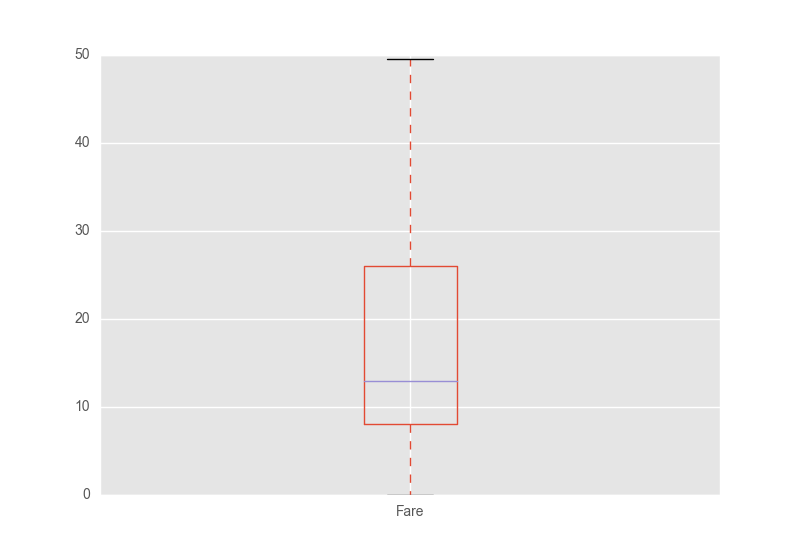
\includegraphics[width=0.7\textwidth]{Images/figure_10.png}
\caption{Gráfico de caja correspondiente a los valores que toma el precio del ticket.}
\end{center}
\end{figure}

Además, se procedió a realizar un histograma que relacione el precio del ticket con la sobrevivencia del pasajero. Esta relación se muestra en la Figura 8.

\begin{figure}[H]
\begin{center}
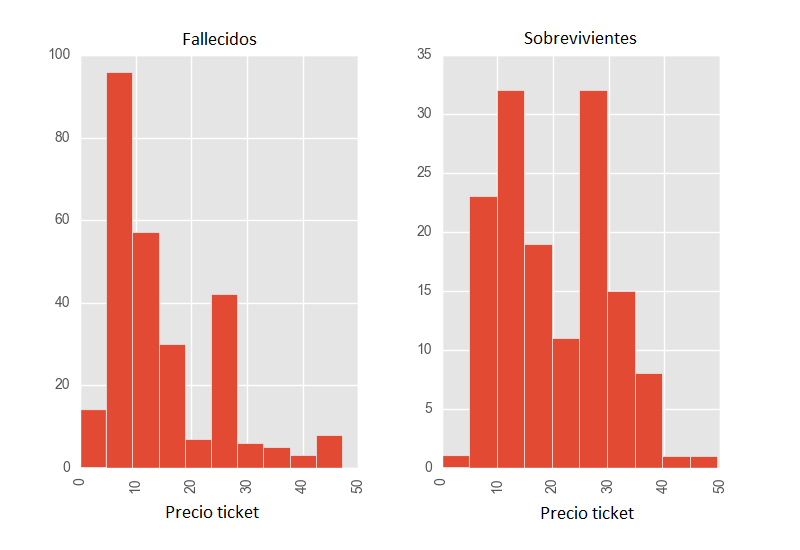
\includegraphics[width=0.7\textwidth]{Images/figure_11.png}
\caption{Gráfico de tipo histograma que muestra la relación existente entre el precio del boleto y la cantidad de personas fallecidas/sobrevivientes.}
\end{center}
\end{figure}

Al juntar ambos gráficos en uno solo, para igualar las escalas y poder comparar de mejor forma si existe una correlación, se generó el gráfico de la Figura 9.

\begin{figure}[H]
\begin{center}
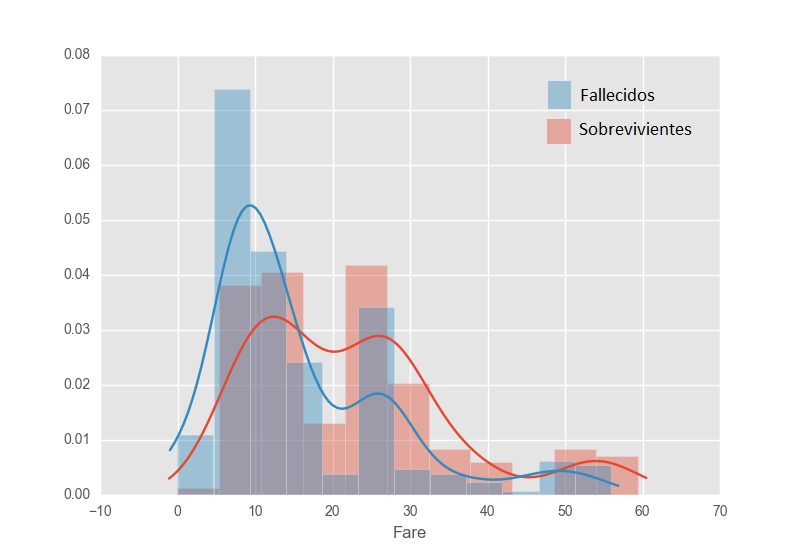
\includegraphics[width=0.8\textwidth]{Images/figure_12.png}
\caption{Histogramas de la variable de sobrevivencia/muerte con respecto al precio del boleto.}
\end{center}
\end{figure}

De este ultimo gráfico, se observa que las personas con ticket de 10 a 20 euros, fallecieron en mayor cantidad que los que sobrevivieron. Los pasajeros con tickets entre 20 y 30 euros, tienen una mayor probabilidad de sobrevivir que de morir, tal como se observa en la curva de color naranja.\\

Luego, se construyó una nueva variable en el dataframe, la cual se forma de 5 intervalos de precios: [0; 9], [10; 19], [20; 29], [29; 39], [40; $\infty$], por lo que la nueva variable llamada \textit{rango}, puede tomar valores enteros del 1 al 5, correspondiente al intervalo en donde se encuentra el precio del boleto. Al agregar esta nueva variable a la predicción realizada anteriormente con la clase y sexo del pasajero, se añadió que además de cumplirse dichos valores, el valor del ticket se encuentre en cualquier intervalo menos en el 2, que es en donde se produce la mayor cantidad de muertes. Esta predicción obtuvo en el dataset de entrenamiento, una precisión de 57,72\% y un recall de 57,89\% para ambos, diferenciándose en sus decimales.\\

Finalmente, se procedió a evaluar ambos métodos predictivos en el dataset de prueba. Para el primer método, tomando solo en cuenta las variables de género y clase del pasajero, se obtuvo una precisión de 68,16\% y un recall del 80,26\%. Mientras que para el segundo método añadiendo el precio del ticket, se logró una precisión del 64,38\% y un recall de 67,76\%.\\

Se puede ver que para ambos métodos, las precisiones y los recall tienen valores muy cercanos, sin embargo, para el primer método, se obtienen porcentajes más altos, siendo éste mejor que el segundo. Esto se puede deber a que la variable rango no está muy relacionada con la probabilidad de sobrevivir.

\section{PCA y Visualización II}

Del conjunto de datos entregado por Gapminder \cite{G1} , para la incidencia del VIH en distintos países del mundo, se eliminan las columnas desde 1979 a 1989, es decir, el análisis queda entre 1990 y 2011. Luego de obtener un dataframe con 139 países y 22 años de evolución de incidencia, se procede a preparar y modelar estos datos para un análisis de componentes principales. Luego de observar el archivo csv dispuesto, se aprecian números notoriamente elevados en países de ubicación  Se presentan a continuación los resultados obtenidos, para un gráfico de líneas comparativo entre distintos países del mundo:

\begin{figure}[H]
\begin{center}
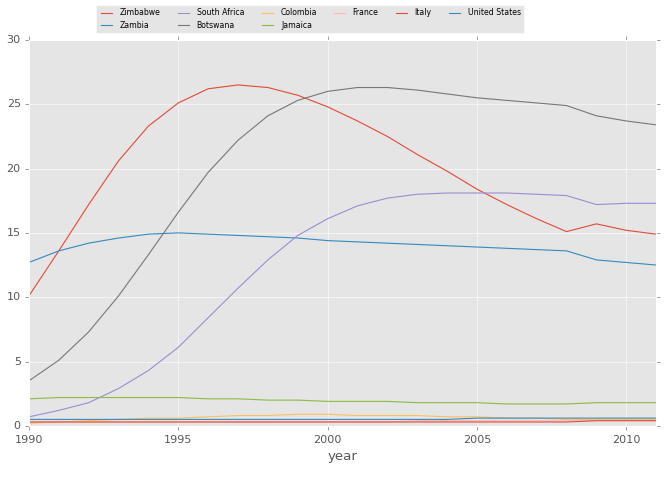
\includegraphics[width=0.8\textwidth]{Images/1line.png}
\caption{Gráfico de líneas comparativo, incidencia del VIH a lo largo del tiempo.}
\end{center}
\end{figure}

De la figura anterior, se aprecia claramente la exagerada incidencia del VIH en países africanos, donde ya pasado 1995 es posible ver los índices más altos en la historia del mundo, es en este mismo año que Zimbabwe tiene el doble de incidencia que sus países hermanos Zambia y Botswana. Zambia presenta una alta incidencia (la mayor en los 90) pero constante, a diferencia de Botswana que en 1999 supera los índices de Zimbabwe y se convierte por lejos en el \textbf{país más afectado por la enfermedad hasta el año 2011}. Por otro lado, las grandes potencias como USA o países europeos quedan lejos de lo anteriormente descrito, al igual que los países sudamericanos cercanos a Chile, observándose una mayor incidencia en \textbf{Colombia}. La isla \textbf{Jamaica}  presenta el doble de íncidencia que los países anteriormente descritos (USA, Europeos y Sudamericanos), a través de todo el intervalo de tiempo analizado.\\

Al utilizar un gráfico de barras para identificar cuales son las componentes principales que describen la varianza de la muestra en cuestión, se puede obtener cuáles de estas componentes serán importantes para el análisis, así como las que pueden despreciarse:

\begin{figure}[H]
\begin{center}
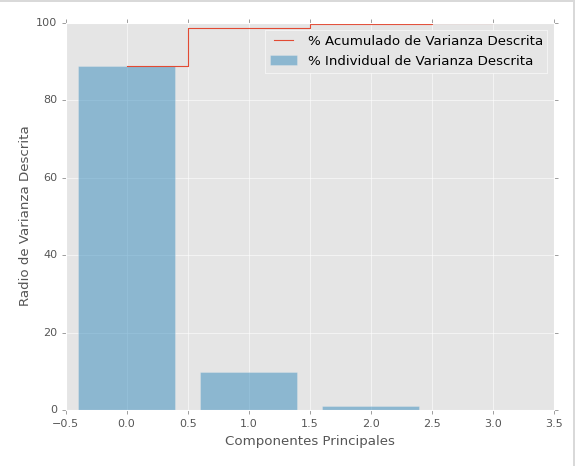
\includegraphics[width=0.8\textwidth]{Images/2var.png}
\caption{Gráfico de barras de la varianza individual y acumulada, primeras 4 PC's, VIH.}
\end{center}
\end{figure}

Es claro ver que \textbf{casi el 90\%} de la varianza de los datos está descrita por la \textbf{primera componente principal}, y que prácticamente la totalidad de la varianza se describe con las dos primeras, por lo que es sano asumir un análisis de dos componentes principales, como la tarea lo especifica.\\

Utilizando un gráfico de puntos con color secuencial para los datos proyectados en sus dos componentes principales, se puede obtener que valores de la componente principal implican la mayor o menor incidencia:

\begin{figure}[H]
\begin{center}
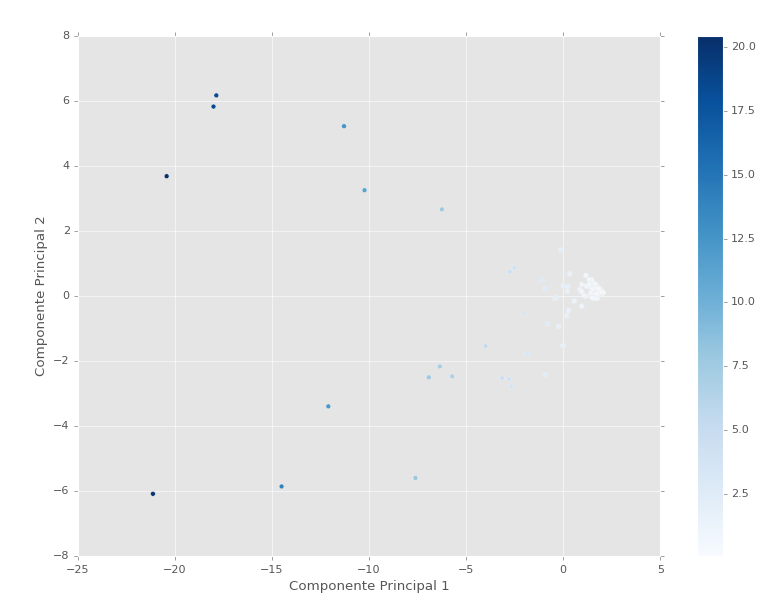
\includegraphics[width=0.7\textwidth]{Images/3scatter1.png}
\caption{Gráfico de puntos, color secuencial de incidencia promedio, VIH.}
\end{center}
\end{figure}

Se observa entonces claramente que la \textbf{primera componente principal codifica la incidencia del VIH}, donde valores de PC1 mayores a 0 tienen casi nula incidencia de la enfermedad. Así para los menores a -10 se asimilan como los países con mayor incidencia total de la enfermedad. Por otro lado, si apreciamos un gráfico de puntos con color divergente, se puede ver qué los países con menor incidencia total, son aquellos que también presentan una disminución con el tiempo:

\begin{figure}[H]
\begin{center}
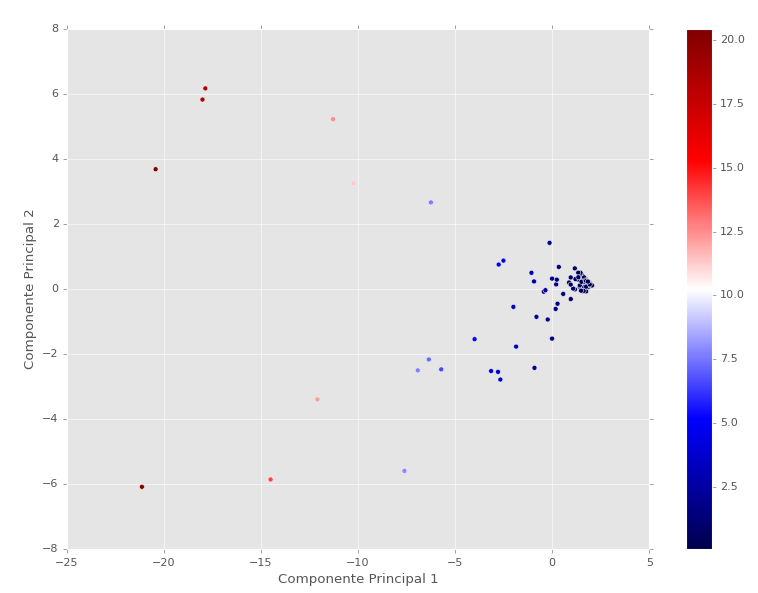
\includegraphics[width=0.6\textwidth]{Images/4scatter2.png}
\caption{Gráfico de puntos, color divergente en incidencia a través del tiempo, VIH.}
\end{center}
\end{figure}

Dado que rojo es disminución y azul aumento (en general), se puede afirmar que los países con PC1 mayor a -5, tienden a disminuir su incidencia, viéndose entre -12 y -5 los países sin mucho cambio, y menos a -12 los que aumentaron su incidencia o bien siguieron con altos índices.\\

De un gráfico de burbujas con color divergente, se puede apreciar la evolución tanto como la incidencia (tamaño), lo que lo convierte en un gráfico más completo para este tipo de análisis. Cuando este se etiqueta, nache la posibilidad de identificar con nombre a outliers y ver continentes mayormente involucrados. Ver a continuación los dos gráficos descritos:

\begin{figure}[H]
\begin{center}
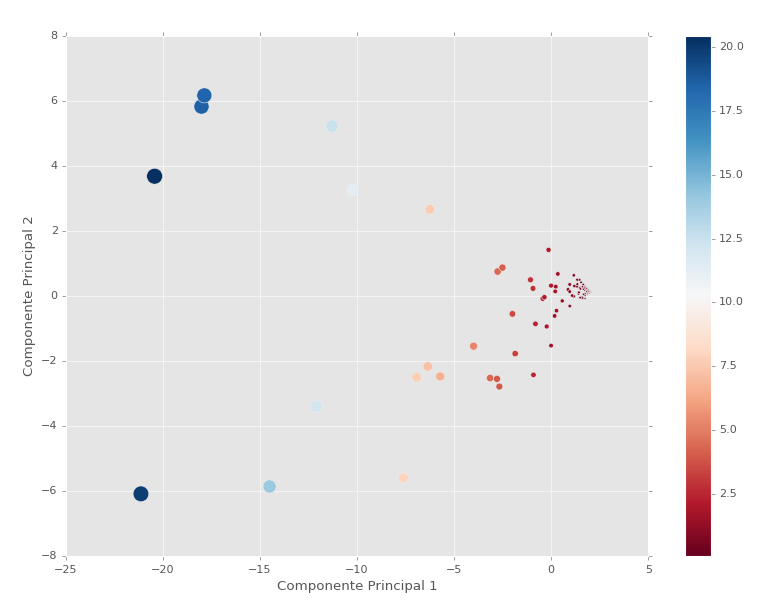
\includegraphics[width=0.6\textwidth]{Images/5bub.png}
\caption{Gráfico de burbujas, color divergente y sin etiquetas, VIH.}
\end{center}
\end{figure}

\begin{figure}[H]
\begin{center}
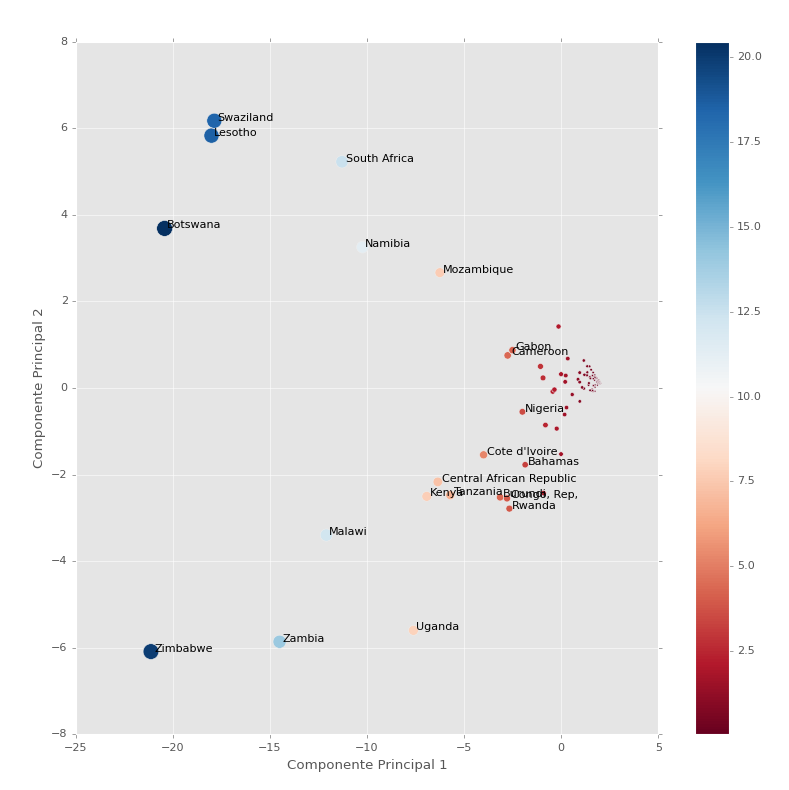
\includegraphics[width=0.6\textwidth]{Images/6bub2.png}
\caption{Gráfico de burbujas, color divergente y etiqueta de país representado, VIH.}
\end{center}
\end{figure}

Se observa finalmente, que para un valor menor a 0 en la PC1, se habla de países africanos en general, con incidencia alta, apareciendo los outliers en valores menores a -10.\\

Luego de estudiar la incidencia del VIH, se pasa a hacer un análisis análogo de los afectados por la Tubercolusis a través del tiempo, esta vez, sin eliminar filas ni columnas.


Se utiliza el mismo gráfico de varianza individual y acumulada explicada por cada componente, obteniendo:

\begin{figure}[H]
\begin{center}
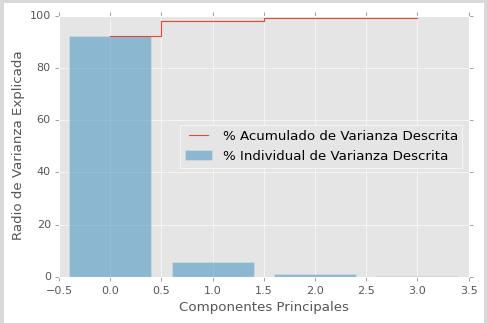
\includegraphics[width=0.8\textwidth]{Images/2-1var.png}
\caption{Gráfico de barras de la varianza individual y acumulada, primeras 4 PC's, TB.}
\end{center}
\end{figure}

Se aprecia que \textbf{más del 90\%} de la varianza de los datos está descrita por la \textbf{primera componente principal}, y que la totalidad de la varianza se describe con las dos primeras.\\

Utilizaremos los gráficos de puntos para obtener valores de la primera componente principal que ayuden a obtener que es lo que decodifica, su magnitud y su evolución:

\begin{figure}[H]
\begin{center}
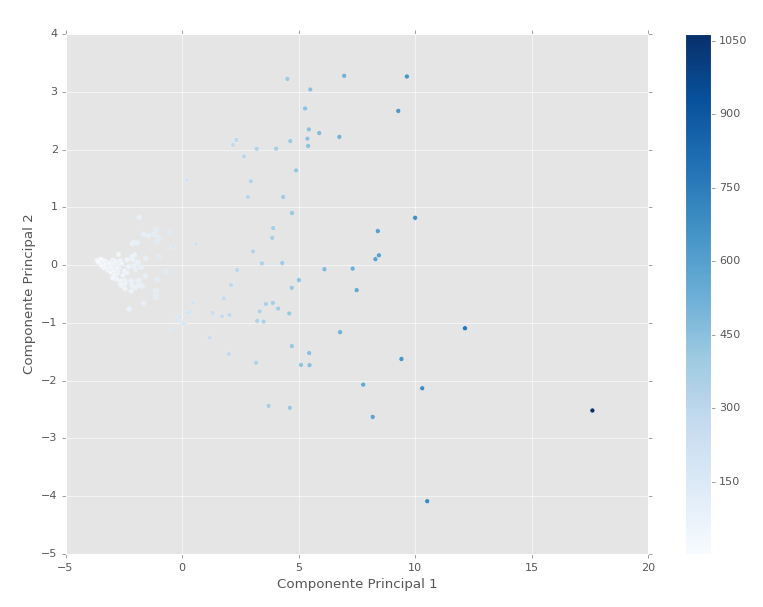
\includegraphics[width=0.7\textwidth]{Images/2-2sca1.png}
\caption{Gráfico de puntos, color secuencial de incidencia promedio, TB.}
\end{center}
\end{figure}

\begin{figure}[H]
\begin{center}
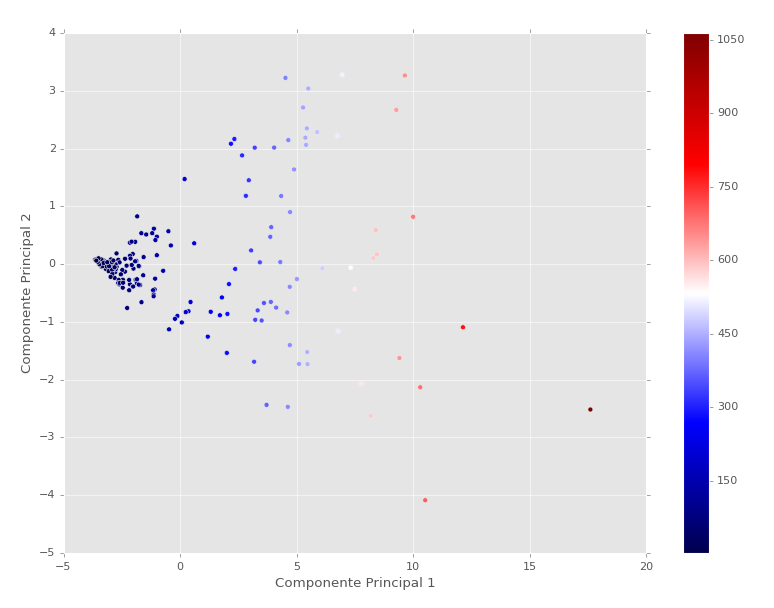
\includegraphics[width=0.6\textwidth]{Images/2-3sca2.png}
\caption{Gráfico de puntos, color divergente en incidencia a través del tiempo, TB.}
\end{center}
\end{figure}

Se observa entonces que al contrario del VIH, valores positivos de la PC1 codifican la cantidad de afectados en los países, viendose los menos afectados en valores negativos, y los más afectados en valores mayores a 10.

Los gráficos de burbuja representan en este caso la cantidad de afectados por el tamaño de la burbuja, y su evolución (disminución roja, aumento azul) a través del tiempo:

\begin{figure}[H]
\begin{center}
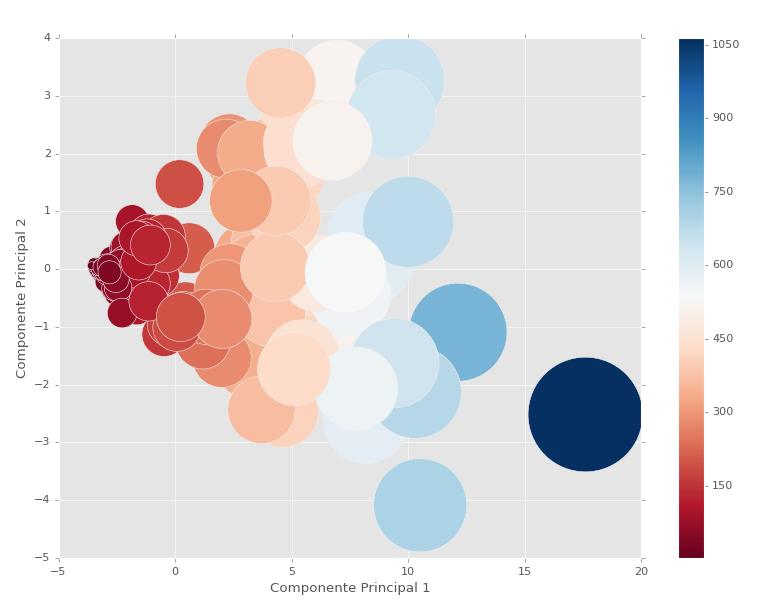
\includegraphics[width=0.6\textwidth]{Images/2-4burb.png}
\caption{Gráfico de burbujas, color divergente y sin etiquetas, TB.}
\end{center}
\end{figure}

\begin{figure}[H]
\begin{center}
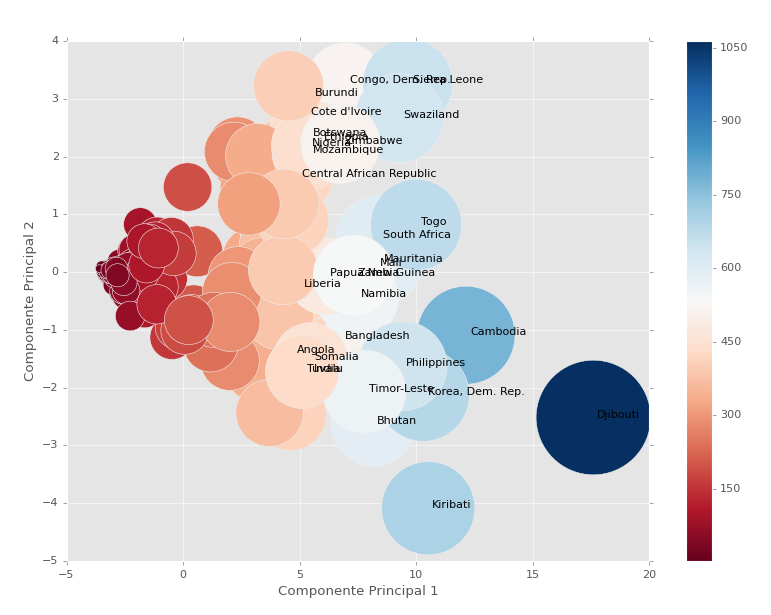
\includegraphics[width=0.6\textwidth]{Images/2-5burb.png}
\caption{Gráfico de burbujas, color divergente y etiqueta de país representado, TB.}
\end{center}
\end{figure}

\bibliographystyle{plain}
\bibliography{Referencias}



\end{document} 